\documentclass[border=10pt]{standalone}
\usepackage{verbatim}
\usepackage{pgfplots}
\pgfplotsset{compat=1.14}

% stars_count = 512;
% max_time = 2.5
% steps = {0.1, 0.1 / 8, 0.1 / (8 * 8), 0.1 / (8 * 8 * 8), 0.1 / (8 * 8 * 8 * 8), 0.1 / (8 * 8 * 8 * 8 * 8)};

\begin{document}

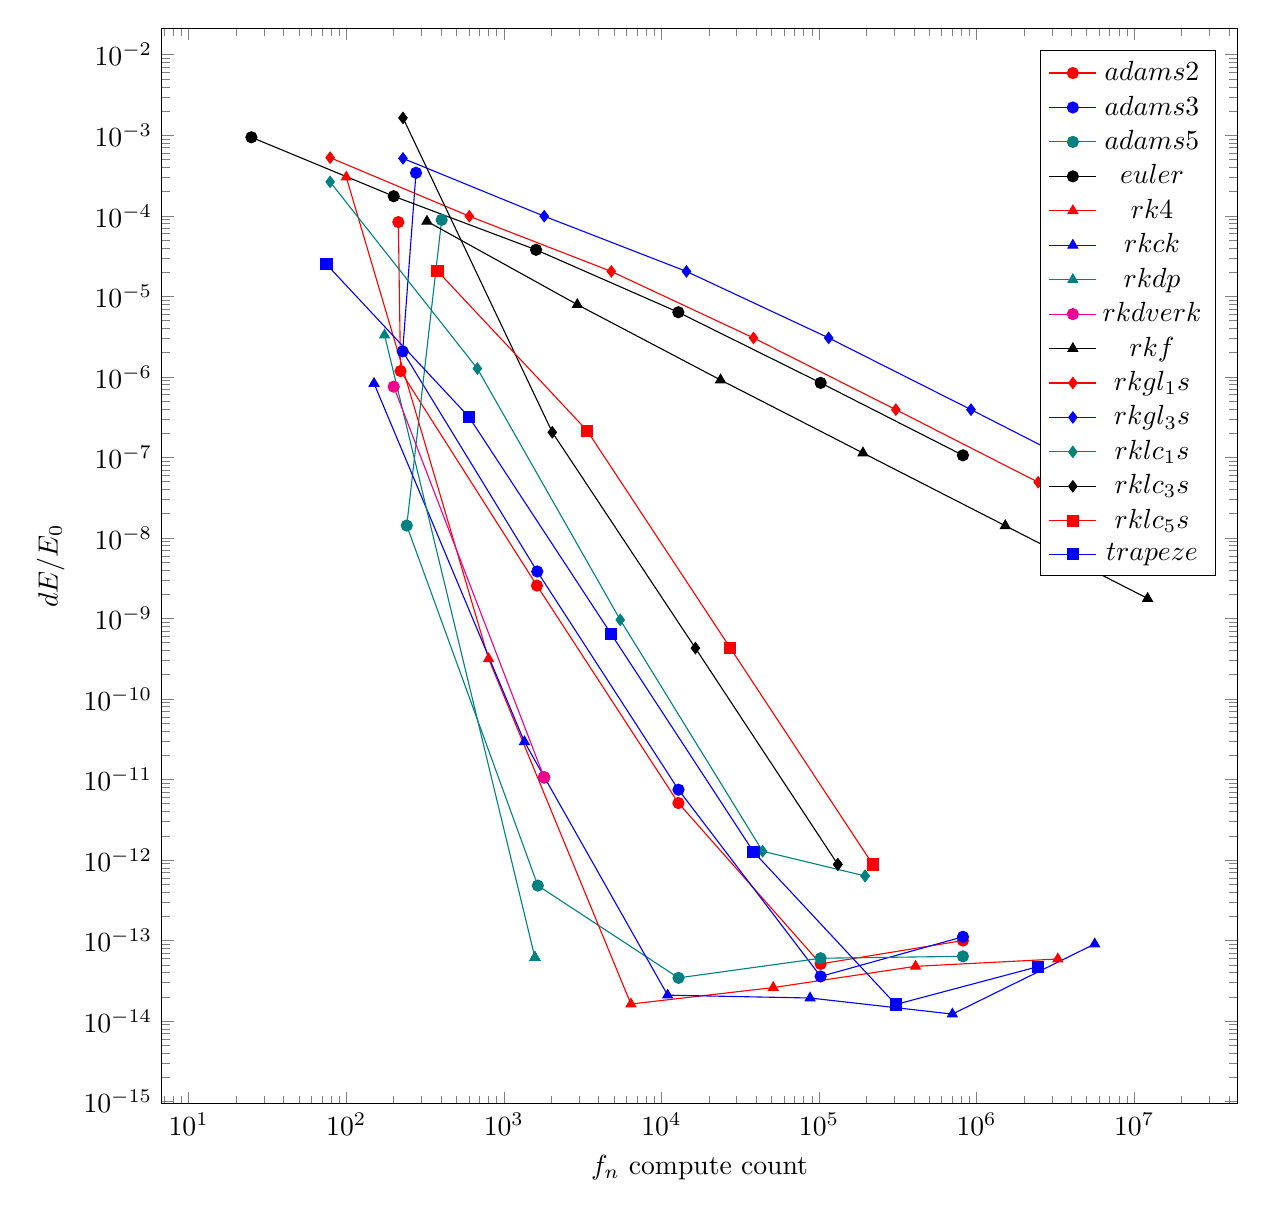
\begin{tikzpicture}
\begin{loglogaxis}[
    height=6in,
    width=6in,
    xlabel=$f_n$ compute count,
    ylabel=$dE/E_0$
]
\addplot [red,mark=*,solid] coordinates { (214, 8.349e-05) (221, 1.18e-06) (1622, 2.558e-09) (1.282e+04, 5.1e-12) (1.024e+05, 5.133e-14) (8.192e+05, 1e-13) };
\addplot [blue,mark=*,solid] coordinates { (277, 0.0003418) (228, 2.076e-06) (1629, 3.829e-09) (1.283e+04, 7.47e-12) (1.024e+05, 3.585e-14) (8.192e+05, 1.114e-13) };
\addplot [teal,mark=*,solid] coordinates { (403, 8.898e-05) (242, 1.424e-08) (1643, 4.817e-13) (1.284e+04, 3.442e-14) (1.024e+05, 6.029e-14) (8.192e+05, 6.375e-14) };
\addplot [black,mark=*,solid] coordinates { (25, 0.0009438) (200, 0.000175) (1601, 3.781e-05) (1.28e+04, 6.342e-06) (1.024e+05, 8.416e-07) (8.192e+05, 1.061e-07) };
\addplot [red,mark=triangle*,solid] coordinates { (100, 0.0003018) (800, 3.161e-10) (6404, 1.629e-14) (5.12e+04, 2.607e-14) (4.096e+05, 4.786e-14) (3.277e+06, 5.906e-14) };
\addplot [blue,mark=triangle*,solid] coordinates { (150, 8.278e-07) (1350, 2.941e-11) (1.095e+04, 2.098e-14) (8.775e+04, 1.935e-14) (7.022e+05, 1.222e-14) (5.617e+06, 9.063e-14) };
\addplot [teal,mark=triangle*,solid] coordinates { (175, 3.303e-06) (1575, 6.131e-14) (1575, 6.131e-14) (1575, 6.131e-14) (1575, 6.131e-14) (1575, 6.131e-14) };
\addplot [magenta,mark=*,solid] coordinates { (200, 7.555e-07) (1800, 1.064e-11) (1800, 1.064e-11) (1800, 1.064e-11) (1800, 1.064e-11) (1800, 1.064e-11) };
\addplot [black,mark=triangle*,solid] coordinates { (325, 8.546e-05) (2925, 7.891e-06) (2.372e+04, 9.153e-07) (1.901e+05, 1.134e-07) (1.521e+06, 1.416e-08) (1.217e+07, 1.77e-09) };
\addplot [red,mark=diamond*,solid] coordinates { (79, 0.0005269) (604, 9.874e-05) (4807, 2.039e-05) (3.841e+04, 3.043e-06) (3.072e+05, 3.916e-07) (2.458e+06, 4.913e-08) };
\addplot [blue,mark=diamond*,solid] coordinates { (229, 0.0005162) (1804, 9.882e-05) (1.441e+04, 2.039e-05) (1.152e+05, 3.043e-06) (9.216e+05, 3.916e-07) (7.373e+06, 4.913e-08) };
\addplot [teal,mark=diamond*,solid] coordinates { (79, 0.0002638) (679, 1.268e-06) (5479, 9.606e-10) (4.388e+04, 1.285e-12) (1.961e+05, 6.342e-13) (1.961e+05, 6.342e-13) };
\addplot [black,mark=diamond*,solid] coordinates { (229, 0.001645) (2029, 2.05e-07) (1.643e+04, 4.279e-10) (1.316e+05, 8.823e-13) (1.316e+05, 8.823e-13) (1.316e+05, 8.823e-13) };
\addplot [red,mark=square*,solid] coordinates { (379, 2.065e-05) (3379, 2.143e-07) (2.738e+04, 4.283e-10) (2.194e+05, 8.815e-13) (2.194e+05, 8.815e-13) (2.194e+05, 8.815e-13) };
\addplot [blue,mark=square*,solid] coordinates { (75, 2.492e-05) (600, 3.184e-07) (4803, 6.388e-10) (3.84e+04, 1.265e-12) (3.072e+05, 1.609e-14) (2.458e+06, 4.746e-14) };
\legend{$adams2$,$adams3$,$adams5$,$euler$,$rk4$,$rkck$,$rkdp$,$rkdverk$,$rkf$,$rkgl_1s$,$rkgl_3s$,$rklc_1s$,$rklc_3s$,$rklc_5s$,$trapeze$};
\end{loglogaxis}
\end{tikzpicture}

\end{document}
